\chapter{Evaluation and Discussion}\label{sec:evaluation}

In this chapter the reference implementation of the conceptual framework is evaluated.
First, a couple of use cases are described and how a geographical visualization can create more value.
A performance evaluation is carried out, to discover technical limitations and to find performance bottlenecks.
As a last step, the requirements of Chapter~\ref{sec:analysis} are used to validate the conceptual framework and the reference implementation.

\section{Use Cases and Discussion}\label{sec:use-case}

The following three use case scenarios demonstrate how more insights can be gained with \gv{} next to the \tmap{}.

\subsection{Explain outliers}\label{sec:evaluation:use-cases:gas-stations}

\tmaps{} can have outliers, i.e.\ unusual local maxima of a certain attribute.
If the attribute is mapped to the height of the corresponding block, a local maximum is identifiable by a block that protrudes from a group of evenly leveled blocks.
We can see such an example in Figure~\ref{fig:evaluation:use-cases:gas-prices}.

The data set of the visualizations in the figure includes gas stations in Berlin.
The \tmap{} is configured as follows:
The layout is based on the brand name of a gas station, i.e.\ gas stations of the same brand like ``Total'' or ``Aral'' are grouped together.
Height and colour of the blocks are mapped to the price of ``Diesel'' and ``E10'' respectively.

A \tmap{} with this configuration is suited to show a correlation of brand and price.
Gas stations of brand ``Total'' are located on the center-left side of the \tmap{} and they are rather expensive in general but with smaller price variations.

This is in strong contrast to gas stations of brand ``ARAL'' in the lower left:
10 gas stations can be identified as outliers, which are more expensive than other gas stations in the group.
``Esso'' and ``Shell'', located in the center and on the lower right, show outliers, too.

Gas stations of the brands ``HEM'', ``Star'' and ``Sprint'' are generally inexpensive and located in the groups with lighter colours at the top and on the right.

However, the \tmap{} alone is not able to explain the reason for certain outliers.
What is special about the protruding blocks, i.e.\ the outliers within a group?

The \gv{} can give a possible explanation:
Many of those outliers are gas stations located next to a highway.
These gas stations are slightly more expensive in general and significantly more expensive if they belong to the brand ``ARAL''.

\begin{figure}
  \centering
  \subfloat[Tree map]{{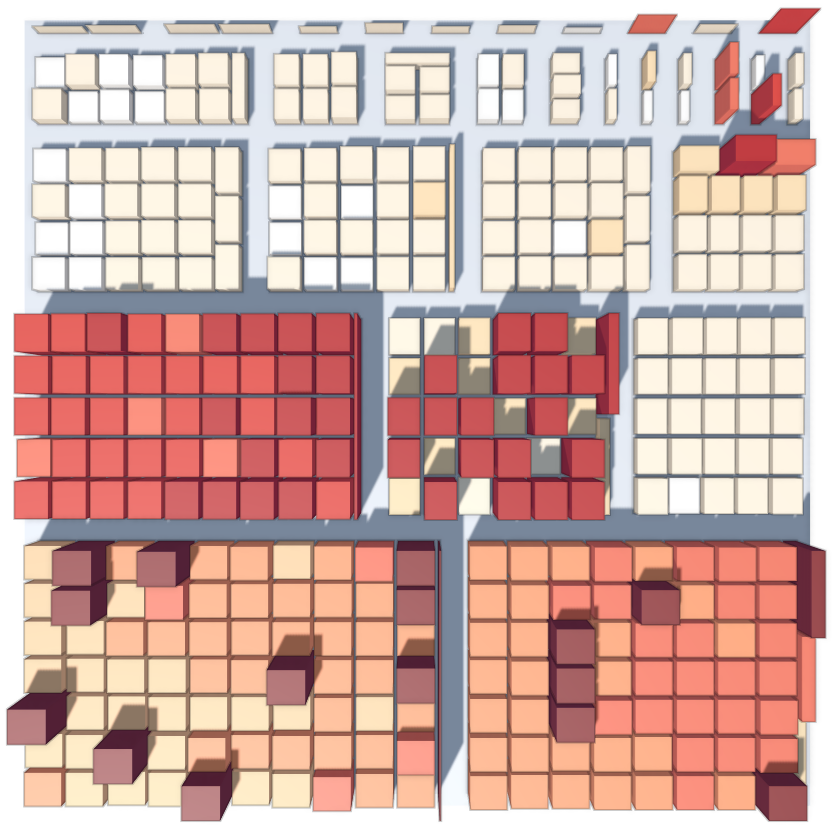
\includegraphics[width=0.4\textwidth]{figures/evaluation/use-cases/1-tmap} }}%
  \qquad
  \subfloat[Point of interest visualization]{{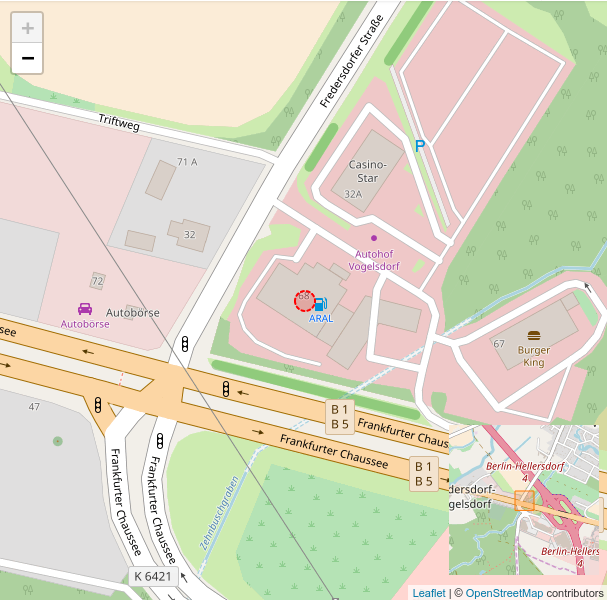
\includegraphics[width=0.4\textwidth]{figures/evaluation/use-cases/1-map} }}%
  \caption{
    Expensive gas stations, compared to other gas stations of the same brand, are often located next to highways.
  }\label{fig:evaluation:use-cases:gas-prices}
\end{figure}

\subsection{Multi-Select in \tmap{}}\label{sec:evaluation:use-cases:multiselect}

This use case demonstrates the benefit of a multiple select and the ability to relate interesting features with their geographic context.
Figure~\ref{fig:evaluation:cases:multiselect:1} (a) shows a \tmap{} with the following configuration:
The layout is based on the population density, large clusters on the right are sparsely populated districts.
Colour is based on the increase or decrease of inhabitants, a red colour indicating a growth of inhabitants.

There are three groups of items in the \tmap{} that catch our interest:
\begin{enumerate*}[label=(\arabic*)]
  \item A group of orange items on the left side of treemap,
  \item many scattered, white coloured items in the large cluster on the right and
  \item three purple coloured items in the large cluster on the right.
\end{enumerate*}

Districts in the orange group are rather densely populated and show a decline of population.
But as we can see in Figure~\ref{fig:evaluation:cases:multiselect:1} (b) the districts of this group have a geographic context:
They are all located in the Ruhr area.

A similar observation can be made about the white group, i.e.\ sparsely populated districts with a serious decline of population:
These districts are all located in the east of Germany, see Figure~\ref{fig:evaluation:cases:multiselect:2} (a).

And finally, even the three purple districts in the cluster of sparsely populated districts are geographically related as well:
These districts are in the vicinity of Munich, as we can see in Figure~\ref{fig:evaluation:cases:multiselect:2} (b).


\begin{figure}
  \centering
  \subfloat[Tree map]{{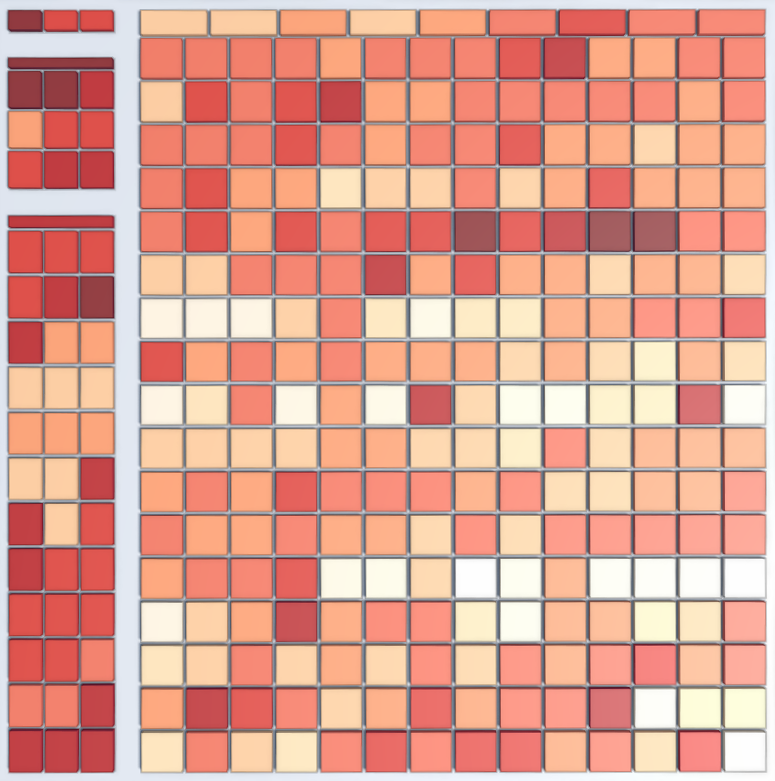
\includegraphics[width=0.4\textwidth]{figures/evaluation/use-cases/2-tmap} }}%
  \qquad
  \subfloat[Orange group]{{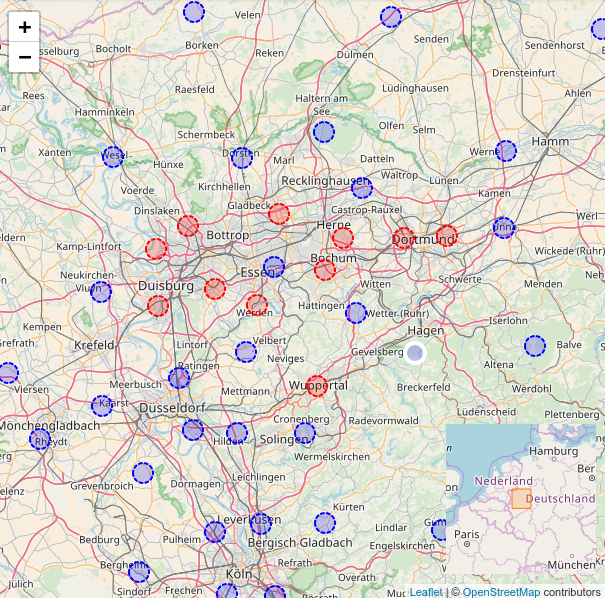
\includegraphics[width=0.4\textwidth]{figures/evaluation/use-cases/2-map-ruhr} }}%
  \caption{
    The orange coloured group on the left, districts with a moderate decline of inhabitants and large population density, are all districts of the Ruhr area.
  }\label{fig:evaluation:cases:multiselect:1}
\end{figure}

\begin{figure}
  \centering
  \subfloat[White group]{{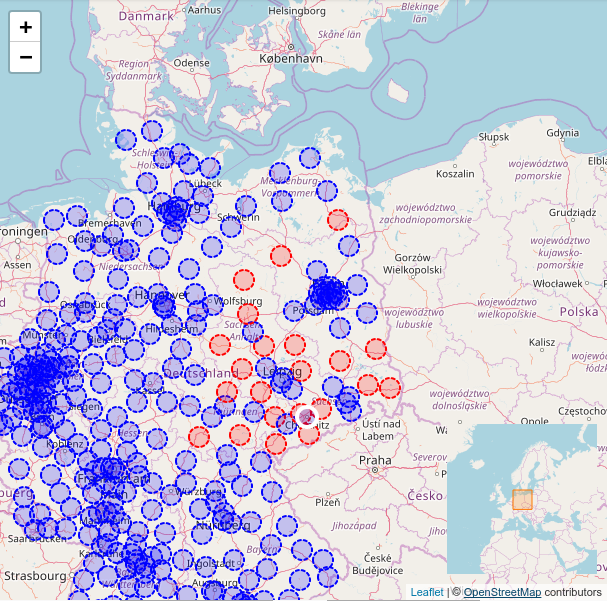
\includegraphics[width=0.4\textwidth]{figures/evaluation/use-cases/2-map-east} }}%
  \qquad
  \subfloat[Purple group]{{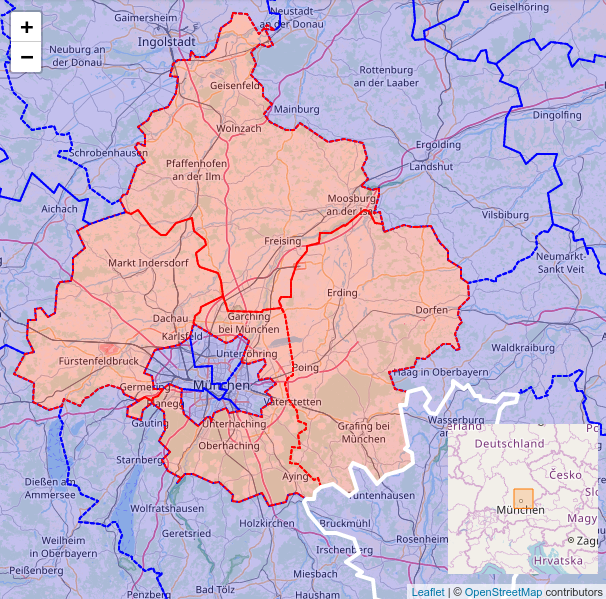
\includegraphics[width=0.4\textwidth]{figures/evaluation/use-cases/2-map-munich} }}%
  \caption{
    The sparsely populated districts with a serious decline of inhabitants are all located in the east of Germany.
    The few districts with a low population density and high increase of population are all located in the vicinity of Munich.
  }\label{fig:evaluation:cases:multiselect:2}
\end{figure}

\subsection{Bounding Box Selection in \gv{}}\label{sec:evaluation:use-cases:bounding-box}
Similar to the multiple select in Section~\ref{sec:evaluation:use-cases:multiselect}, multiple selects can be carried out by a bounding box in the \gv{}.

The layout of the \tmap{} in Figure~\ref{fig:evaluation:cases:bounding-box} (a) is based on construction activity, i.e.\ the number of completed accommodations per capita.
The colour is mapped to the increase of population.
As Berlin is known for quickly rising rents and real estate speculation we select all districts in Berlin with a bounding box.
All selected districts are placed in the center right group of the \tmap{}.
They are the dark red items next to the currently highlighted item in Figure~\ref{fig:evaluation:cases:bounding-box} (a).
But as we can see in Figure~\ref{fig:evaluation:cases:bounding-box} (a), the districts are not in the group with the highest construction activity at the very top.

\begin{figure}
  \centering
  \subfloat[Tree map]{{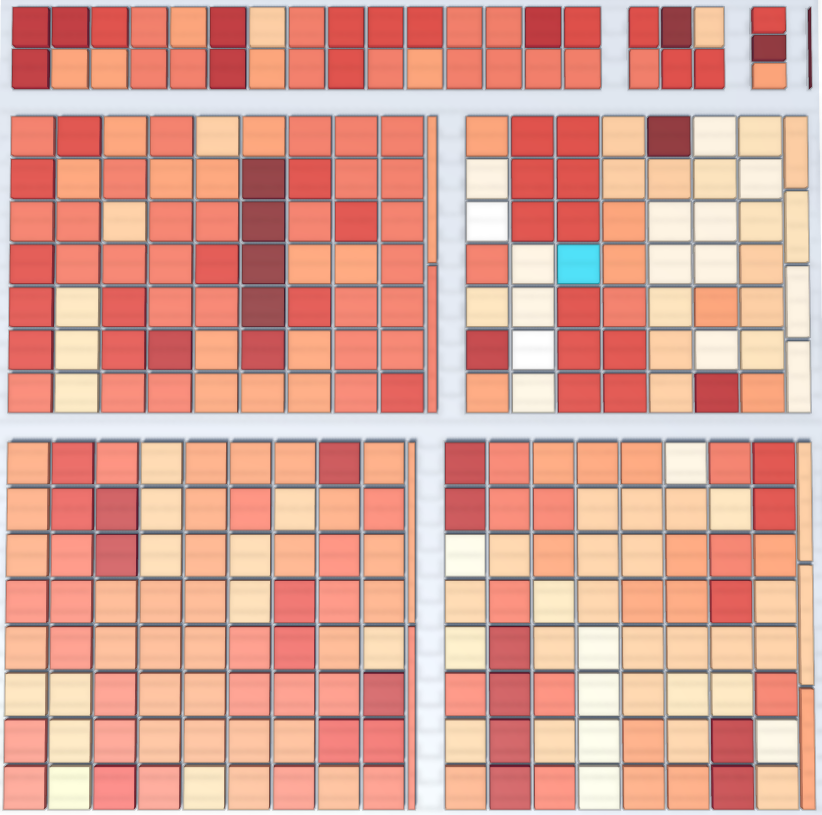
\includegraphics[width=0.4\textwidth]{figures/evaluation/use-cases/3-tmap} }}%
  \qquad
  \subfloat[Geographic map]{{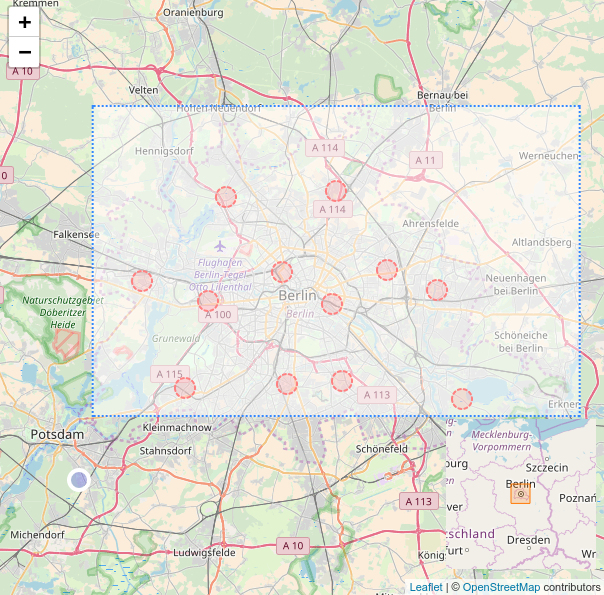
\includegraphics[width=0.4\textwidth]{figures/evaluation/use-cases/3-map} }}%
  \caption{
    A bounding box multiple select in the \gv{} can reveal a non-geographic context in the \tmap{}
  }\label{fig:evaluation:cases:bounding-box}
\end{figure}

\subsection{Use case summary}

The scenario in Section~\ref{sec:evaluation:use-cases:gas-stations} is a great example how a \gv{} can create more insights.
The \tmap{} alone allows to identify the outliers and also shows a possible correlation of price and brand.
However, without the \gv{} it is not possible to draw a hypothesis of the proximity to a highway being the reason for the high prices.
The geographic context is just not present in the raw data.

Deliberately selecting a particular area of interest in the \gv{} by clicking on an interesting item in the \tmap{} can be considered to be a new technique.

Similarly, in the scenario in Section~\ref{sec:evaluation:use-cases:multiselect}, the \tmap{} alone can show outliers or group of outliers.
However, it is not possible to see the geographic relation between those items in that group immediately.
The \gv{} makes the geographic context visible.
In this scenario, the multiple selection really helps to select items of the white group, which is scattered across the \tmap{}.

Finally, in the scenario of Section~\ref{sec:evaluation:use-cases:bounding-box}, we can also do the reverse:
Identify a non-geographic relation in the \tmap{} by selecting geographically related items with a bounding box.
In this case we can see a very similar construction activity.


\section{Performance Evaluation and Limitations}

The following performance evaluation was carried out with the built-in runtime performance analysis feature of the Chrome browser.
In particular, a Chromium Browser was used in Version 62.0 (64 Bit).
The hardware specifications of the machine are listed in Table~\ref{tab:evaluation:performance:hardware}.

\begin{table}[ht]
  \centering
  \caption{Hardware specifications.}%
  \label{tab:evaluation:performance:hardware}
  \begin{tabular}{ll}
    Device name: & LENOVO ThinkPad L540 \\
    CPU type: & Intel i3-4100M CPU @ 2.50GHz \\
    \#CPUs: & 4 \\
    Main memory: & 8GiB \\
    Graphics card: & Intel 4th Gen Core Processor Integrated Graphics Controller \\
  \end{tabular}
\end{table}

A couple of data sets were used in three different scenarios:
\begin{enumerate*}[label=(\arabic*)]
  \item The \tmap{} without a geographical visualization, just publishing interactions,
  \item an example application of the geographical visualization without a \tmap{} and
  \item both visualizations together.
\end{enumerate*}

In the first and second scenario, the data set is loaded, some data points are highlighted and then some data points are focused with a single-select and a multi-select holding the control-key.
In the second scenario and third scenarios, which have a geographical visualization, we also select many items with a select box, holding the shift-key.
For every scenario there are six data sets, that is 18 profilings, and each scenario profiling took about 60 seconds to finish.

Table~\ref{tab:evaluation:performance:data-sets} shows the list of data sets used for profiling the performance of the reference implementation.
The largest data set consists of German administrative districts called ``Landkreise Deutschland'' with a total size of 2.13 MiB.
The data set with the highest number of features is called ``Immoscout Wohnungsangebote'' with 8601 coordinates German real estates, totalling 2.11 MiB.

\begin{table}[ht]
  \centering
  \caption{Data sets used for performance profiling.}%
  \label{tab:evaluation:performance:data-sets}
  \begin{tabular}{lllr}
    Data Set & Features & Type & Size (MiB) \\
    \hline
    Bundesländer Deutschland      & 16   & Areas  & 0.64 \\
    Tankstellen Berlin            & 366  & Points & 0.75 \\
    Wahlkreise BT 2009            & 299  & Areas  & 0.91 \\
    Regierungsbezirke Deutschland & 31   & Areas  & 0.94 \\
    Immoscout Wohnungsangebote    & 8601 & Points & 2.11 \\
    Landkreise Deutschland        & 402  & Areas  & 2.13 \\
  \end{tabular}
\end{table}


\subsection{Immoscout}
The slowest profiling is the visualization of data set ``Immoscout''.
Chrome's runtime analysis shows a red bar at the top of the screen if the frames per second drop in such a way that it impairs the perceived interactivity.
You can see a screenshot of the analysis in Figure~\ref{fig:evaluation:performance:profiling:immoscout:fps}.


\begin{figure}[ht]
  \centering
  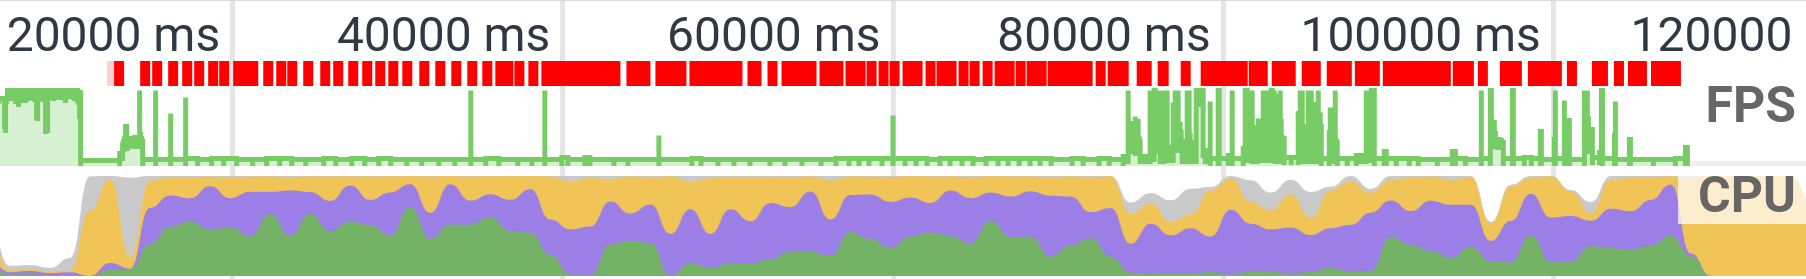
\includegraphics[width=\textwidth]{figures/evaluation/performance/profiles/immoscout_both/fps}
  \caption{During profiling of both \tmap{} and \gv{} visualizing the ``Immoscout'' data set, the frame per second rate drops to 1 FPS.}
  \label{fig:evaluation:performance:profiling:immoscout:fps}
\end{figure}

As you can see in Figure~\ref{fig:evaluation:performance:profiling:immoscout:summary} the \tmap{} spends almost the entire CPU time in scripting.
The \gv{} has a more balanced CPU time, spending time for painting and rendering during focusing interactions.

\begin{figure}[ht]
  \centering
  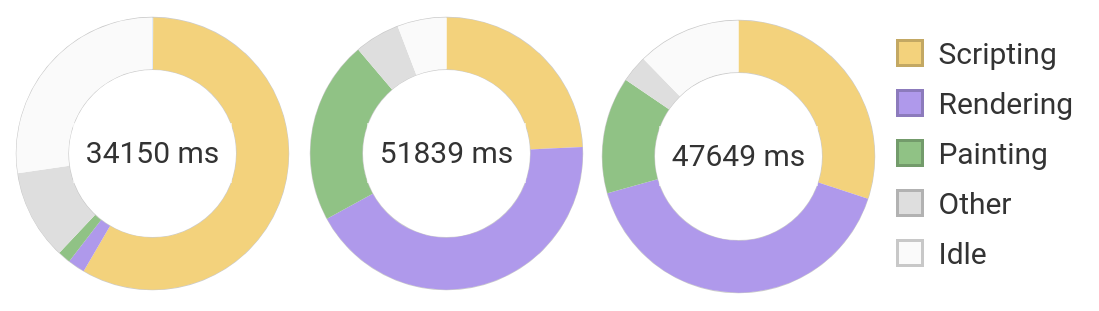
\includegraphics[width=\textwidth]{figures/evaluation/performance/summaries/immoscout}
  \caption{
    Summary of profile data for data set ``Immoscout'' of \tmap{} only (left), both \tmap{} + \gv{} (center) and only \gv{} (right).
  }\label{fig:evaluation:performance:profiling:immoscout:summary}
\end{figure}

Going through the timeline, we can identify the handling of the ``mousemove'' event to be the likely cause of this slow scripting.
The \tmap{} constantly checks the point or polygon which is under the mouse cursor.
This is likely a performance problem.

The profile summary looks totally different for the scenario of a \tmap{} along with a \gvis{}.
Compared to just a \tmap{} only, much more time is spent during painting and rendering.
This is caused by the fact, that LeafletJS moves the viewpoint and zooms if a feature is focused.
This can cause a network request and will re-render background tiles.

Note that not the communication between views hits the performance but rather the change of visual representation of views.


\begin{figure}[ht]
  \centering
  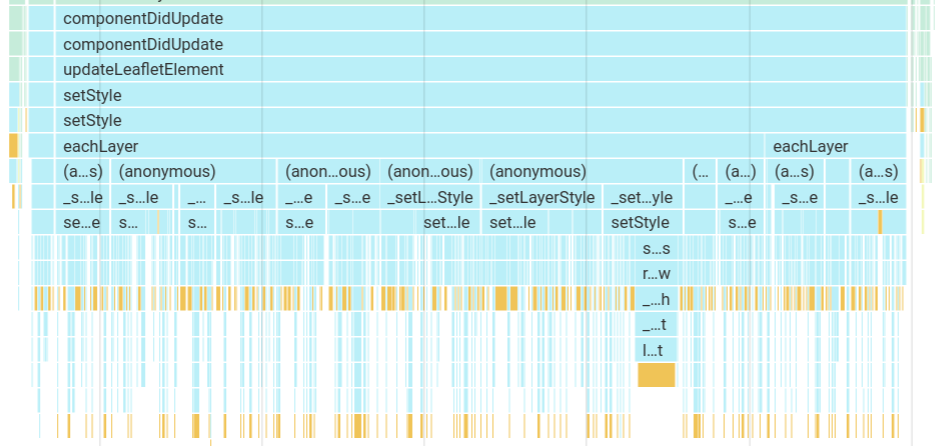
\includegraphics[width=\textwidth]{figures/evaluation/performance/profiles/immoscout_geo_only/callstack}
  \caption{
    The sawtooth pattern of the callstack during a \attr{highlight} interaction indicates an expensive iteration of all features of the \attr{GeoJSON}.
  }\label{fig:evaluation:performance:profiling:immoscout_both:callstack}
\end{figure}


Figure~\ref{fig:evaluation:performance:profiling:immoscout:fps} shows spikes whenever an interaction is made.
Most of these interactions are \attr{highlight} interactions, when the user moves the mouse cursor.
Figure~\ref{fig:evaluation:performance:profiling:immoscout_both:callstack} shows the lower part of the callstack during such a \attr{highlight} interaction.

We can identify the dominating subroutine to be \attr{setStyle} which spans almost the entire callstack.
Below this subroutine, you can see a lot of quick calls for each layer.
\attr{LeafletJS} iterates through all geographic features in order to update the style, e.g.\ change the stroke width.
Therefore, \attr{setStyle} seems to be costly operation for a large number of features.
This would explain why many small features have a stronger performance impact than fewer but larger features.


\subsection{Landkreise}
The profiling of data set ``Landkreise'' seems to support that assumption.
This data set is larger than ``Immoscout'' but has fewer features.
Nevertheless, the frame per second rate rarely drops in a way which has an impact on interactivity, as you can see in Figure~\ref{fig:evaluation:performance:profiling:landkreise_both:fps}.


\begin{figure}[ht]
  \centering
  \caption{
    Larger but fewer features seem to have positive effects on the frame rate.
  }\label{fig:evaluation:performance:profiling:landkreise_both:fps}
  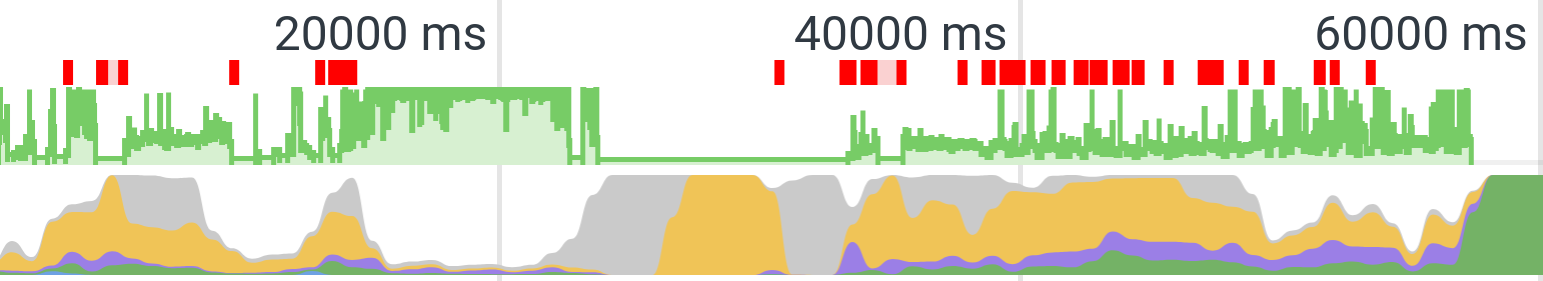
\includegraphics[width=\textwidth]{figures/evaluation/performance/profiles/landkreise_both/fps}
\end{figure}

The \gv{} alone idles almost 50\% of the CPU time, as you can see on the right side of Figure~\ref{fig:evaluation:performance:profiling:landkreise:summary}.
\begin{figure}[ht]
  \centering
  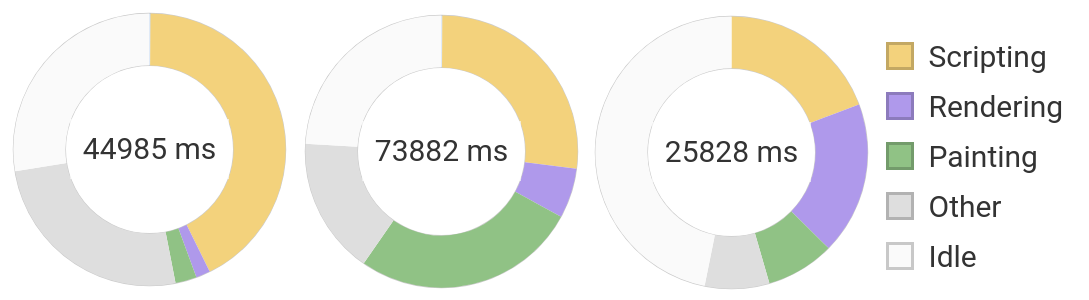
\includegraphics[width=\textwidth]{figures/evaluation/performance/summaries/landkreise}
  \caption{
    Summary of profile data for data set ``Landkreise'' of \tmap{} only (left), both \tmap{} + \gv{} (center) and only \gv{} (right).
  }\label{fig:evaluation:performance:profiling:landkreise:summary}
\end{figure}



\section{Evaluation of Requirements}\label{sec:evaluation:requirements}
In this section, the reference implementation is evaluated based on the requirements from Section~\ref{sec:analysis:requirements}.

\textbf{Serialization} of interactions depends on the published interaction data.
The interaction type is just a string and therefore trivial to serialize.
But the payload of the interaction can be an arbitrary JavaScript object, so the serialization depends on the serialization of that data.

In our case, the largest JavaScript object that is published as interaction data are the geometries during initialization.
This step is necessary as there is no shared state of data between visualizations and every view needs to hold its own data.
Only identifiers are valid across multiple views, but each view is allowed to have its own internal structure of data.

The largest data set of geometries at hand is called ``Immoscout Wohnungsangebote'' and consists of 8617 geographical features with a total size of 2.1 MB on disk.
These geometries are stored as GeoJSON, i.e.\ \gls{json}.

After the initialization, data transmission between views can be reduced by exchanging implicit functions instead of explicit data sets.
E.g.\ if some data points shall be hidden, the threshold function can be published instead of a set of entity ids that are hidden.
In JavaScript, functions can be serialized with \attr{toString()} and deserialized with \attr{eval}.


\textbf{Reversibility} of interactions also does not depend on the interaction framework but rather on the implementation of the participating visualizations.
The undoing of an interaction needs to be implemented in each view separately.
If the interaction framework is used to publish an \attr{undo} interaction, there are two possible implementations:
\begin{enumerate*}[label=(\arabic*)]
  \item
    Each visualizations keeps a record of every past interaction and can replay the record up to the desired step
    \item
    or the mathematical inverse of the function is published.
\end{enumerate*}
Both options have an undesired impact on the required memory, because data needs to be kept in memory for every visualization.
If the record of interactions is long, the first implementation will take a long time to replay every interaction up to the desired state.

If past interactions are mathematically reversible, e.g.\ a threshold function for a filter interaction, the \attr{undo} interaction only needs to publish the inverse function.
The number of interactions does not have an impact on the performance, but if more than just one interaction shall be reversed, a record of past interactions need to be stored.

\textbf{Data extensibility} of interactions is enabled with arbitrary JavaScript objects.
In Section~\ref{sec:analysis:requirements} good extensibility is present when
\begin{enumerate*}[label=(\arabic*)]
  \item
    additional data attributes can be added without lookup of corresponding items and
  \item
    no de-duplication steps are necessary when new items are added.
\end{enumerate*}
Since every entity in the data set is considered to be identifiable, a lookup of additional data can be accomplished a request with the entity id.
Entity ids are unique, so no de-duplication is necessary.
Since attributes have a unique name, the value of an attribute for the entity can be replaced without de-duplication.

\textbf{Development costs} do not diminish significantly.
The framework design assumes loose coupling, independent views and no shared state.
It is lightweight, has a low complexity and scales well.
The downside of this approach is that it does not come with a huge simplification of implementing visual changes and event handlers in single views.
Implementing the correct trigger and effect of interactions stays to be the main burden of work.

\textbf{Maintainability} as described in Section~\ref{sec:analysis:requirements} means how much other parts of the code are impacted by an interaction and how error-prone the framework is.
The framework benefits of the main advantages of the publish-subscribe pattern, i.e.\ loose coupling and scalability.
On the other hand, it suffers from the main disadvantages of this software pattern, the decoupling of publisher and subscriber.
Debugging the connections can be quite cumbersome and the asynchronous publishing can lead to further errors.

The geographical visualization is 873 lines long which is quite small.
The glue code of a very simple example takes 132 lines of code.

% \subsection{Data Sets}
% For our uses cases, we have two different data sets:
% One data set consists of a user ranking of public broadcasting in Germany, i.e.\ entities, mostly TV and radio broadcasts, are liked or disliked by people.
% This data is public data and can be used by media researchers of broadcasting corporations but also targets media journalists and the general audience.
% The other set, called \riso{}, consists of statistical data from various German administrations and is used by the authorities for urban planning and policy strategies.

% Both data sets share some characteristics.
% The administrative data connects certain features with certain regions of Germany.
% As Germany is a federal state, larger regions consist of many other smaller regions.

% The second one consists of user data that was collected through a web application called \rufu{}.

% \subsubsection{RISO}

% The \riso{} data base is used in by local authorities to get insights about governmental KPIs to assist local and regional decision making.
% It is a relational database and a part of the data base schema is shown as an ER diagram in Figure~\ref{fig:data:riso}.

% \begin{figure}[ht]
%   \centering
%   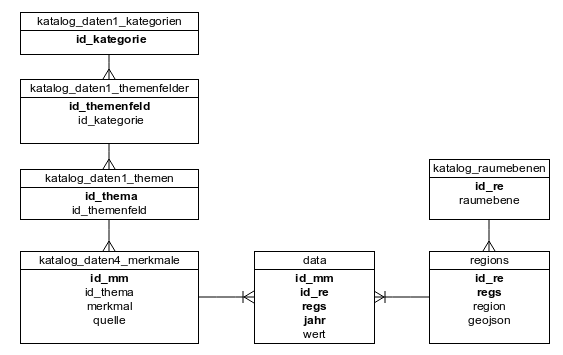
\includegraphics[width=\textwidth]{images/riso}
%   \caption{Part of the \riso{} database schema. Primary keys are set in bold.}\label{fig:data:riso}
% \end{figure}

% The largest table is called \attr{data} with approximately 10,466,600 records, which holds all values along with the survey date.
% \textbf{Features}
% This data is connected to a feature table through a foreign key called \attr{id_mm}.
% In the feature table we can find the description for every referenced feature, e.g.\ population density, working population in agriculture, education spending.
% The \riso{} system groups all features in a 4-level hierarchy:
% \begin{enumerate}
%   \item
%     \attr{katalog_daten_1_kategorien}
%   \item
%     \attr{katalog_daten_2_themenfelder}
%   \item
%     \attr{katalog_daten_3_themen}
%   \item
%     \attr{katalog_daten_4_merkmale}
% \end{enumerate}
% The actual features table is the last one in the list.
% At the lowest level within the hierarchy, this is the largest table with 1234 records.


% \textbf{Regions}
% On the other side, the geographical data is stored in the \attr{regions} table.
% The geometry data for each region is stored in the \attr{geojson} column and as the name suggests, the data type is a \attr{geojson}.
% The foreign keys that connect the tables \attr{data} and \attr{regions} are called \attr{id_re} and \attr{regs}.
% Unlike the feature table, the regions are grouped through the \attr{id_re} that indicates the hierarchy level.
% So the values of the \attr{id_re} column denominate the level of the hierarchy.
% E.g.\ a region with a \attr{id_re} of $1$ is a federal state of Germany, a region with id $13$ is a constituency.
% A textual description for the hierarchy level can be found in the \attr{katalog_raumebenen} table in column \attr{raumebene}.
% Both column \attr{id_re} and \attr{regs} belong to the primary key of the regions table, so there will never be two regions on the same hierarchy level with the same \attr{regs} id.

% \textbf{Characteristics}
% As we can see, the schema of the \riso{} database follows a rather denormalized approach.
% The schema does not make a lot of assumptions regarding the input data.
% It allows to add data of arbitrary size, features and completeness as long as there is some kind of numerical data associated with some kind of geographical unit.
% This approach is suitable for a data base that incorporates data from different sources, as it is the case with the \riso{} data base.


% \subsubsection{\rufu{}}
% Unlike the \riso{} database, the data base of \rufu{} is used as persistence layer.
% For that reason the data base schema follows the requirements of a web application in production.

% As outlined in Section~\ref{sec:outline} \rufu{} is an evaluation platform for public broadcasting in Germany.
% First, users vote on broadcasts, i.e.\ they decide if they want to support broadcast or if they do not want to support.
% As a next step, user can define a weighting by distributing a virtual, monthly budget among the chosen broadcasts.

% Figure~\ref{fig:data:rundfunk} shows the data base schema of the application.
% A \attr{user} is connected to \attr{broadcast} through a \attr{selection}.
% If the \attr{user} supports some a broadcast, the \attr{response} on the given \attr{selection} will be `positive'.
% If the \attr{user} does not wish to support a \attr{broadcast}, the \attr{response} will be `neutral'.
% The \attr{user} can allocate virtual money to supported broadcasts.
% The money will be stored in the column \attr{amount} of the \attr{selection}.
% The sum of all amounts for one user will never exceed the virtual budget of 17.50€.

% \begin{figure}[ht]
%   \centering
%   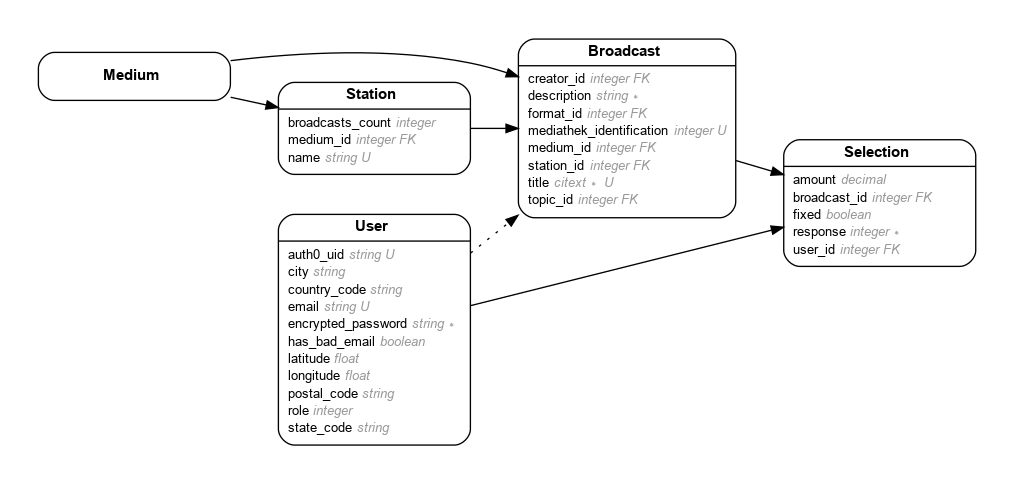
\includegraphics[width=\textwidth]{images/er}
%   \caption{Database schema of the \rufu{} application}\label{fig:data:rundfunk}
% \end{figure}

% \textbf{Features}
% We have both numerical as well as nominal features.
% A numerical feature could be the number of supporters from an area in Germany.
% A nominal feature could be a list of the most supported broadcasts from an area in Germany.
% Numerical and nominal features can be combined, so we could request for every region, a distribution of the desired expenditure for radio, TV, online and other broadcasts.

% \textbf{Regions}
% \rufu{} stores the geometry for each region in \attr{geojson} files.
% These files hold a \attr{FeatureCollection}.
% Every \attr{Feature} is a region, the identifier is stored as a property.
% We merge the geometry data with features for every request.
% To be precise: We get all the user data, group it by the identifier \attr{state_code} and merge it with the geometry in the \attr{geojson}.

% \textbf{Characteristics}
% The data base schema is a result of the specific requirements of the persistence layer.
% Changes in the source code may require a migration of the data base schema.

% However, we can ask a lot of questions already with common data base queries or standard data analysis tools:
% \begin{enumerate}
%   \item
%     How does the actual support of a broadcast compare to the average support of a broadcast?
%   \item
%     What are the most popular broadcasts in Berlin?
%   \item
%     What is the desired ratio of genres of supported broadcasts? How important is education compared to sport?
%   \item
%     How does the support of a broadcast change over time?
%   \item
%     According to the user ranking, which broadcasts are similar to each other?
% \end{enumerate}



% \section{Planned Interactions}
% We have a focus on coordinated multiple views consisting of a treemap and a geographical map.
% Let's have some examples how an interaction between a \tmap{} and a \map{} might work:

%     \begin{enumerate}
%       \item
%         User selects a feature set from the drop down in the menu. This will trigger a \emph{Reconfigure} interaction. A data set consisting of all features and their ids, geometries and metadata is transferred. The receiving components are both the \tmap{} and the \map{} which will rerender the entire visualization.
%       \item
%         User hovers with a mouse over a polygon in the \map{}. This will trigger a \emph{Select} interaction. The data is a single feature id that will be transferred to the \tmap{}, which will change the color of an box.
%       \item
%         Rotate or zoom the \tmap{}. This will also rotate or zoom the \map{}. The interaction would fall into \emph{Explore} and the shared information is the orientation of the camera and the zoom level.
%       \item
%         A click in the \tmap{} will trigger an \emph{Explore} interaction. The data is a single feature id sent to the \map{}. The map will center the viewport on the center of geometry of the respective feature.
%       \item
%         The user selects many features at once in the \map{} by dragging a rectangle. The ids of all features within the rectangle are sent to the \tmap{}. All features will be highlighted with a different color, which is therefore a \emph{Select} interaction.
%       \item
%         \emph{Reconfigure} the layouting of the \tmap{} by choosing a different hierarchy level. This increased granularity may lead to an increased granularity in the \map{}, e.g.\ show postal codes instead of federal states. The changed data are additional items, that are nested in the former items.
%       \item
%         \emph{Encode} the \tmap{} by a different attribute mapping like color, height or texture. If the \map{} has no geometry data that defines the shape of a feature, it can also display a larger point marker.
%       \item
%         Apply a \emph{Filter} and reduce the data set by choosing only items with metadata beyond a certain treshold. The reduced data leads to a full re-render of all data visualizations. The message contains the updated item list
%   \item
%     Show a \emph{Connect} by highlighting boxes of the same subtree in the \tmap{}. The respective connected items would be highlighted in the \map{} as well. Here the data is a relation between items.
%     \end{enumerate}
% \todo[inline]{What are the key interactions in our use case?}

